% Written for Danu.fi, 2022

% I really dislike Beamer

\documentclass{article}

	\usepackage{unicode-math}
	\usepackage{microtype}

	\usepackage{xcolor}

	\usepackage{tikz}
	\usepackage{pgfplots}

	\usepackage{fancyhdr}
	\usepackage{hyperref}
	\usepackage{caption}
	\usepackage{enumitem}

	\usepackage[
		paperwidth = 128mm,
		paperheight = 96mm,
		margin = 1cm,
	]{geometry}

	\usetikzlibrary{
		backgrounds,
		calc,
		external,
		fadings,
		fit,
		positioning,
		shadows,
		svg.path
	}

	\title{Towards optimal AMMs for NFTs}
	\author{Danu}
	\date{\today}

	\definecolor{grayscale-200}{HTML}{595959}
	\definecolor{grayscale-600}{HTML}{dddddd}
	\definecolor{grayscale-700}{HTML}{ebecee}
	\definecolor{grayscale-800}{HTML}{f8f8f8}
	\definecolor{branding-100}{HTML}{6443c6}
	\definecolor{branding-800}{HTML}{ebe6f8}
	\definecolor{branding-900}{HTML}{ebe6f8}

	\tikzfading[
		name = fade out,
		inner color = transparent!0,
		outer color = transparent!100
	]

	% Courtesy of FontAwesome
	% TODO fix coloring, rather than this ugly solution
	\newsavebox{\logomarkbox}
	\savebox{\logomarkbox}{%
		
\begin{tikzpicture}%
			\fill [yscale = -1] svg "m 446.53147,33.43 c -6.86,-37.2 -39.34,-65.43 -78.53,-65.43 -39.23,0 -71.72,28.29 -78.54,65.54 C 126.75147,48.96 -0.4985316,186.12 0.0014684,352.98 0.1114684,387.9 29.081468,416 64.001468,416 H 368.00147 c 8.84,0 16,-7.16 16,-16 0,-17.67 -14.33,-32 -32,-32 h -79.49 l 35.8,-48.33 c 24.14,-36.23 10.35,-88.28 -33.71,-106.6 -23.89,-9.93 -51.55,-4.65 -72.24,10.88 l -32.76,24.59 c -7.06,5.31 -17.09,3.91 -22.41,-3.19 -5.3,-7.08 -3.88,-17.11 3.19,-22.41 l 34.78,-26.09 c 36.84,-27.66 88.28,-27.62 125.13,0 10.87,8.15 45.87,39.06 40.8,93.21 l 118.53,125.94 h 90.38 c 8.84,0 16,-7.16 16,-16 0,-17.67 -14.33,-32 -32,-32 h -53.63 l -98.52,-104.68 154.44,-86.65 a 58.16,58.16 0 0 0 29.71,-50.73 c 0,-21.4 -11.72,-40.95 -30.48,-51.23 -40.56,-22.22 -98.99,-41.28 -98.99,-41.28 z m -78.53,38.57 c -13.26,0 -24,-10.75 -24,-24 0,-13.26 10.74,-24 24,-24 13.25,0 24,10.74 24,24 0,13.25 -10.75,24 -24,24 z";
		\end{tikzpicture}%
	}

	\newcommand{\logo}[1][black]{%
		\tikz{%
			\node at (0, 0) {\resizebox{!}{1.25em}{\usebox{\logomarkbox}}} node [anchor = west, xshift = 2.00em, color = #1] {\normalfont\mbseries\large Danu};
		}
	}%

	\newcommand{\mbseries}{\fontseries{mb}\selectfont}

	\makeatletter%
		\def\@maketitle{%
			\let\footnote\thanks%
			{\parindent0pt%
				\begin{tikzpicture}[remember picture, overlay]%
					\clip [preaction = {
						fill = grayscale-800
					}] (current page.north west) rectangle (current page.south east);%
					\fill [branding-800, path fading = fade out] (current page.north west) circle (5cm);
				\end{tikzpicture}%
				\logo[black]%
				\null%
				\vskip 1cm%
				{\large\mbseries Improving NFT liquidity\par}%
				{\Large\mbseries\@title\par}%
				\vskip 1.5em%
				{\color{grayscale-200}\@date\par}%
				\vspace{\fill}%
				{\hfill\color{grayscale-200}Visit us at \href{https://danu.fi}{danu.fi}}
			}%
			\@thanks%
		}%
	\makeatother%

	% #1 is optional flushright flag, #2 the subtitle, #3 the title
	\newenvironment{formattedslide}[3][false]{
		\newpage%
		{%
			\parindent 0pt%
			\mbseries%
			#2\\[0.25em]%
			{\large #3}\par%
		}
		\vspace{\fill}
		\color{grayscale-200}
	}{
		\vspace{\fill}
	}

	\unimathsetup{
		warnings-off = {
			mathtools-colon, mathtools-overbracket  % No need; obvious
		}
	}
	\defaultfontfeatures{
		Ligatures = TeX,
		Scale = MatchLowercase,
	}
	\setmainfont{Akzidenz Grotesk}[
		Extension = .ttf,
		UprightFont = Akzidenz_Grotesk_Pro_Regular,
		ItalicFont = Akzidenz_Grotesk_RegularItalic,
		FontFace = {mb}{n}{Akzidenz_Grotesk_Pro_Medium},
		BoldFont = Akzidenz_Grotesk_Bold
	]
	\setmonofont{Pragmata Pro Mono}[
		UprightFont = * Regular,
		ItalicFont = * Italic,
		BoldFont = * Bold,
		BoldItalicFont = * Bold Italic
	]
	\setmathfont{STIX Two Math Regular}
	\SetProtrusion{%
		encoding = *
	}{%
		\textquotedblleft = {1000, },%
		\textquotedblright = { ,1000},%
		( = {1000, },%
		) = { ,1000},%
	}

	\tikzset{%
		every text node part/.style = {
			align = center
		},
		block/.style = {
			draw,
			rectangle,
			minimum height=3em,
			minimum width=3em,
			inner sep = 0.5cm
		},
		drawmultiple/.style = {%
			double copy shadow = {%
				shadow xshift=4pt,%
				shadow yshift=4pt,%
				fill=white,%
				draw,%
				draw opacity=#1
			}%
		},%
		drawmultiple/.default=1
	}

	\pgfplotsset{%
		compat=newest,
		danubrandedplot/.style = {
			height = 0.6\textwidth,
			width = \textwidth,
			grid = none,
			axis lines = left,
			axis on top,
			unit rescale keep size,
			axis background/.style = {%
				fill = grayscale-800,
			},
			axis line style = -latex,
			no markers,
			legend columns = 1,
			legend style = {%
				legend pos = north east,
				fill = white,
				fill opacity = 0.8,
				text opacity = 1,
				draw = none,
				column sep = 4pt,
				row sep = 10pt,
			},
			legend cell align = left,
			every tick label/.style = {%
				grayscale-200
			},
			every axis label/.style = {%
				font=\small\mbseries,
			}
		},
	}

	\fancypagestyle{plain}{
		\fancyhf{}
		\fancyfoot[C]{\normalfont\footnotesize\color{grayscale-200}\thepage}
		\renewcommand{\headrulewidth}{0pt}
		\renewcommand{\footrulewidth}{0pt}
	}

	\pagestyle{plain}

	\hypersetup{
		unicode,
		colorlinks = true,
		allcolors = branding-100,
		pdfstartview = FitV
	}

	\setlength{\footskip}{10.25pt}  % minimum

	\linespread{1.15}

	\captionsetup{font={footnotesize, color=grayscale-200, stretch=1.15}}

	\newlist{advantages}{itemize}{1}
	\setlist[advantages]{label={\(\rightarrow\)}}%, leftmargin=0pt}

	\begin{document}

		% Front matter
		\tikzexternaldisable
			\maketitle
			\thispagestyle{empty}
		\tikzexternalenable

		\begin{formattedslide}{Why exist?}{Which problems do we want to solve?}
			\begin{enumerate}
				\item Interest in NFTs is waning, as demonstrated by \href{https://nairametrics.com/2022/07/22/nft-trading-volume-slumps-by-64-in-q2-2022/}{64 \% less volume in Q2}
				\item Lack of consensus on correct NFT pricing leads to volatility and scarcity
				\item Liquidity within NFT collections is also distributed very unevenly\ldots
			\end{enumerate}
		\end{formattedslide}

		\begin{figure}
	\begin{tikzpicture}
		\begin{axis}[
			danubrandedplot,
			xmin = 0,
			xmax = 9,
			xtick = {0, ..., 9},
			xlabel = {Number of transactions},
			enlarge y limits = {rel = 0.1, upper},
			ylabel = {Percentage of collection sold},
			ytick = {0, 50, 100},
			extra y ticks = {39},
			extra y tick labels = {\textcolor{branding-100}{\(\mathbf{39}\)}},
			table/col sep = comma,
			domain = 0:9,
			legend pos = south east,
		]

			% Background traces
			\foreach \j in {1, 2, ..., 20}{
				\addplot [
					thin,
					grayscale-600,
					forget plot
				] table [
					x = count,
					y = n_trades,
				] {data/frequencies/\j.csv};
			}
			\addlegendimage{thin, grayscale-600};
			\addlegendentry{Individual collections};

			% Median, taken from Python script (ask Anis)
			\addplot [very thick, branding-100] table [
				x = count,
				y = n_trades
			] {data/frequencies/median.csv};
			\addlegendentry {Median};
			% Cumulative fraction
			\addplot [
				black,
				densely dotted,
				every axis plot post/.append style = {
					mark = x,
					mark options = {
						solid
					}
				}
			] coordinates {
				(0, 39.3)
				(1, 68.0)
				(2, 84.4)
				(3, 92.9)
				(4, 96.5)
				(5, 98.2)
				(6, 98.9)
				(7, 99.0)
				(8, 99.1)
				(9, 99.2)
			};
			\addlegendentry{Cumulative median};
		\end{axis}
        \end{tikzpicture}
        \caption{Pareto chart of the percentage of collections sold, including e.g. \href{https://boredapeyachtclub.com/}{Bored Ape Yacht Club (BAYC)}, for the twenty most-traded PFP-based collections on \href{https://opensea.io}{OpenSea}. 39 \% of indexed collections do not trade at all and 29 \% exchange hands only once.}
        \label{fig:characteristic_normalized_price}
\end{figure}



		\begin{formattedslide}{The solution}{What do we propose?}
			If we could wave a magic wand, how would we improve the situation?

			\begin{advantages}
				\item Build an AMM for NFTs, with a marketplace front-end à la \href{https://opensea.io}{OpenSea}
				\item Incentivize sustainable liquidity with tokenomics, à la \href{https://filecoin.io}{Filecoin} or \href{https://chain.link}{Chainlink}
			\end{advantages}

			\textbf{This scheme would provide liquidity instantly, as well as a marketplace to discover and trade exceptional NFTs on.}
		\end{formattedslide}

		\newsavebox{\pricingoraclebox}
\savebox{\pricingoraclebox}{%
	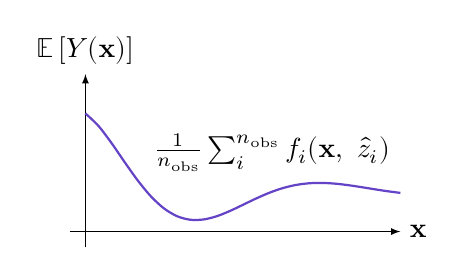
\begin{tikzpicture}
		\draw [very thin, -latex] (-0.2, 0) -- (4, 0) node[right] {$\mathbf{x}$};
		\draw [very thin, -latex] (0, -0.2) -- (0, 2) node[above] {$\mathbb{E}\left[{Y(\mathbf{x})}\right]$};
		% sin(\x r + 180)) + 0.8, otherwise underdamped oscillator
		\draw [thick, smooth, branding-100] (0, 0) plot [domain=0:4] (\x, {exp(-0.7*\x)*cos(2*\x r + 0.2) + 0.5}) node [black, above, anchor = south east, yshift=4pt] {$\frac{1}{n_\text{obs}} \sum_i^{n_\text{obs}} f_i(\mathbf{x},~\hat{z}_i)$};
	\end{tikzpicture}%
}


\newsavebox{\tokens}
\savebox{\tokens}{%
	
\begin{tikzpicture}
		\path (-0.75, 0.2) rectangle (0.95, -1.85);  % Compensate paddings for drawmultiple
		\draw [
			fill = white,
			drawmultiple,
		]
			(0.75, 0) --
			(-0.75, 0) --
			(-0.75, -1.75) --
			plot [
				domain=0:1.5,
				xshift=-0.75cm,
				yshift=-1.75cm
			] ({\x}, {0.1*sin(4*\x r + 180)}) -- cycle;
			%\node at (0, -0.875) {Tokens \\ \(\mathbb{T}_◌\)};
	\end{tikzpicture}
}


\newsavebox{\smartcontract}
\savebox{\smartcontract}{%
	\begin{tikzpicture}
		\node (tokens-1) at (0, 0) {\usebox{\tokens}};
		%\node [
		%	right = of tokens-1,
		%	xshift = -0.75cm
		%] (tokens-2) {\usebox{\tokens}};
		\begin{scope}[on background layer]
			\node [
				fill = grayscale-700,
				fit = (tokens-1)(tokens-1),
				inner sep = 5mm,
				label = {[%
					anchor = west,%
					xshift = 2.5mm,%
					fill = white
				]north west:Liquidity pool \(i\)}
			] (pool) {};  % https://tex.stackexchange.com/questions/59012/how-to-use-fit-to-frame-the-nodes-and-labels
		\end{scope}

		\begin{scope}  % Compensate for double draw offset
			\node [xshift = -1mm] at (tokens-1) {Tokens \\ \(\mathbb{T}_i\)};
		\end{scope}
	\end{tikzpicture}
}


\begin{figure}
	\centering
	\begin{tikzpicture}[
		node distance = 1.00cm and 1.50cm,
		label distance = 5mm,
		component/.style = {%
			draw,
			fill = white,
			inner sep = 2.5mm
		}
	]

		% Components
		% - Pricing DS
		\node [
			component,%
			label = {[name = labelDS] Open-source NFT pricing model},%
			drawmultiple = {0.2}
			] (DS) at (0, 0) {\usebox{\pricingoraclebox}};
		% - Exchange smart contract
		\node [
			component,
			right = of DS
		] (SC) {\usebox{\smartcontract}};
		\node [component, densely dashed, above = of SC] (Users) {Users (LPs and takers)};

		% Arrows
		\draw [<->] (SC.north) -- (Users.south) node [midway, fill=white] {\footnotesize Commissions};
		\draw [->] (DS.east) -- (SC.west) node [midway, fill=white] {\footnotesize TTP};

	\end{tikzpicture}
	%\caption{Lorem ipsum dolor sit amet, consectetur adipiscing elit. Sed molestie lorem a dui porttitor fermentum. Aliquam aliquet est vel ipsum lobortis pharetra. In efficitur nec ex in cursus.}%
	%\caption{One of our novelties is to use an off-chain pricing model as a mediator in transactions. That way, liquidity providers (LPs) accrue less risk and traders obtain much more accurate pricing than with the established solution of bonding curves.}
	\caption{One of our novelties is the use of an off-chain pricing model in transactions, as opposed to the established solution of using bonding curves. That way, liquidity providers (LPs) accrue less risk and traders obtain much more accurate pricing.}
	\label{fig:architecture}
\end{figure}



		\begin{formattedslide}{The solution}{Embracing the superiority of off-chain pricing models}
			Why not use an on-chain NFT appraisal model à la \href{https://sudoswap.xyz}{Sudoswap}, or a variation thereof? Because off-chain pricing models\ldots

			\begin{advantages}
			% uniswap v2 vs v3
			\item allow vulnerabilities to be patched without \href{https://medium.com/coinmonks/uniswap-v2-vs-v3-by-the-numbers-10b37124b087}{fragmenting liquidity} and can be \textbf{updated dynamically}.

			For example, even if an on-chain model had \(R^2\approx0.99\) now, who is to say that will always remain the case?
			\item are \textbf{gas-optimal}, as gas price is independent of model complexity. Models can therefore also be arbitrarily complex
			\item readily allow securities and API dependencies to be built upon them with \textbf{blockchain-agnostic} and \textbf{automatic price updates}
			\end{advantages}
		\end{formattedslide}

		\begin{formattedslide}{The solution}{But doesn't this go against the DeFi ethos?}
			No, to the contrary! We think it's time to finally start viewing the blockchain as a means to an end, rather than the end-goal itself.

			From a standpoint of pragmatism, if the model is open-source, verifiable, much more secure, faster (think of e.g. database indexes), and distributed, why \emph{not} allow it to complement the deficiencies of blockchains?\\

			\textbf{Our best-of-both-worlds approach allows for a level of performance and flexibility that on-chain NFT-AMMs can never achieve.}
		\end{formattedslide}

		\begin{formattedslide}{The solution}{In other words\ldots}
			\begin{tikzpicture}[remember picture, overlay]
				\node[
					grayscale-600,
					scale=7.5
				] at ($(current page.east) + (-1.5cm, 0)$) {''};
			\end{tikzpicture}
			``If a concern can possibly be addressed outside of a smart contract, then that’s what we should do.\makebox[0pt][l]{''}
			\vskip0.5em%
			\hspace\fill--- \href{https://medium.com/solidified/b67fb4073422}{R. Hitchens}
		\end{formattedslide}

		\begin{formattedslide}{The solution}{Mainnet pricing model}
			Our mainnet NFT appraisal model\ldots
			\begin{advantages}
			\item is \textbf{open-source}, audited, and thoroughly motivated in documentation
			\item provides \textbf{reliable prices} to our traders and API customers
			\item implements a \textbf{risk premium} (RP), to ameliorate systemic and idiosyncratic risk and protect our LPs
			\end{advantages}

			%and, while still requiring considerable research effort in our opinion, already manage to achieve an \(R^2\approx0.81\).

			And yes, we will pay out bounties for every merged considerable improvement!
		\end{formattedslide}

		\begin{figure}
	\centering
	\begin{tikzpicture}[
		every node/.style = {
			text width = 0.275\textwidth,
			inner sep = 0pt,
			outer sep = 0pt,
		},
		node distance = 1mm and 1mm
	]%
		% Row 1
		\node (d1) {\includegraphics[width=\linewidth]{img/devilish-1}};
		\node [right = of d1] (d2) {\includegraphics[width=\linewidth]{img/devilish-2}};
		% Row 2
		\node [below = of d1] (kf1) {\includegraphics[width=\linewidth]{img/kung_fu-1}};
		\node [below = of d2] (kf2) {\includegraphics[width=\linewidth]{img/kung_fu-2}};
	\end{tikzpicture}
	\caption{The NFT appraisal model can be run ``in reverse'', as statistically-optimal generative models for a given set of traits and art styles. To be released as several collections on mainnet. Why cats and not frogs? Because we're saving the best for last\ldots}%
	\label{fig:reverse}
\end{figure}



		\begin{formattedslide}{Testnet}{Differences between testnet \& mainnet}
			\begin{description}
			\item [Simplified pricing model] The testnet is not representative of the real world. We therefore chose to demonstrate our pricing model using a toy example on one collection, as to not create unrealistic expectations.

			\item [No guaranteed liquidity] As a consequence of the above, we do not have an appropriate tokenomics model for testnet behavior. After six months, even our mainnet tokenomics are to be fine-tuned.

			\item [No optimizations or regards to security] The code is meant to be understood easily, while being written in the allotted time.
			\end{description}

			But what it \emph{can} do, is demonstrate the viability of the off-chain NFT-AMM beyond any reasonable doubt.
		\end{formattedslide}

		% back matter
		\newpage
		\vspace*{\fill}
		{\parindent 0pt%
			{\mbseries\large Check out the demo at \href{https://testnet.danu.fi/marketplace}{testnet.danu.fi/marketplace}\\}%

			\textcolor{grayscale-200}{For more information, check out our \href{https://danu.fi/light_paper.pdf}{light paper}.}
		}
		\vspace{\fill}

		% Care to learn more? Read our lite paper and contact us

	\end{document}


